\chapter{METODOLOGÍA DE LA INVESTIGACIÓN}
\section{Diseño de la investigación}
En esta sección del documento se explicará cual es el diseño, el tipo y el enfoque del trabajo de
investigación, así como también la población y la muestra. 
%Para finalizar se explicará el
%proceso de aplicación de las redes neuronales convolucionales.
\subsection{Enfoque de la investigación}
El presente trabajo tendrá un enfoque cuantitativo ya que se busca diseñar y desarrollar instrumentos, en este caso modelos predictivos, para responder al problema estudiado a partir de medición de datos históricos en la plataforma Kickstarter con herramientas basadas en la estadística y matemáticas que puedan ser interpretadas por cualquier investigador. 

\subsection{Alcance de la investigación}
El alcance del presente trabajo será descriptivo ya que se recolectarán datos en un determinado rango de tiempo (desde 2009 hasta el presente año 2019) para describir el comportamiento de las campañas de proyectos tecnológicos en Kickstarter a partir de las características de sus variables y con ello, pronosticar su posible éxito o fracaso antes de finalizar la campaña con un nivel óptimo de precisión.

\subsection{Tipo de la investigación}
Para determinar el tipo de la investigación, primero es necesario definir el actual trabajo como Diseño Experimental ya que las variables que se tienen serán controladas, es decir, serán agregadas o quitadas en el o los modelos construidos en el experimento para analizar el impacto que este o estos tendrán en los resultados obtenidos. Dentro de esta categoría se clasifica como Diseño Experimental Puro ya que se busca medir la variable dependiente, en este caso Status (el estado actual del proyecto en Kickstarter) a partir de la manipulación de las demás variables independientes agregando o desagregándolas para comparar los rendimientos obtenidos de los instrumentos de medición y determinar cuáles de ellas finalmente serán tomadas en cuenta.

\subsection{Descripción del prototipo de investigación}
Teniendo como referencia investigaciones basadas en Aprendizaje Profundo Multimodal, es decir, que combinan distintas características de una campaña de crowdfunding (\citeauthor{pr_kamath2018suplearn}, primer antecedente; \citeauthor{pr_jin2019dayssuccess}, noveno antecedente; \citeauthor{pr_cheng2019deeplearning}, décimo antecedente) usando Metainformación (\citeauthor{pr_kamath2018suplearn}, primer antecedente; \citeauthor{pr_beckwith2016predcrowd}, segundo antecedente; \citeauthor{pr_zhou2015projectdesc}, tercer antecedente; \citeauthor{pr_yuan2016textanalytics}, cuarto antecedente; \citeauthor{pr_chen2015predcrowd}, quinto antecedente; \citeauthor{pr_li2016predcrowd}, sexto antecedente; \citeauthor{pr_kaur2017socmedcrowd}, séptimo antecedente; \citeauthor{pr_yu2018deeplearning}, octavo antecedente; \citeauthor{pr_jin2019dayssuccess}, noveno antecedente; \citeauthor{pr_cheng2019deeplearning}, décimo antecedente; \citeauthor{pr_mitra2014phrases}, duodécimo antecedente; \citeauthor{pr_sawhney2016usingLT}, decimotercer antecedente; \citeauthor{pr_chen2013kickpredict}, decimocuarto antecedente), descripción del proyecto (\citeauthor{pr_zhou2015projectdesc}, tercer antecedente; \citeauthor{pr_yuan2016textanalytics}, cuarto antecedente; \citeauthor{pr_jin2019dayssuccess}, noveno antecedente; \citeauthor{pr_cheng2019deeplearning}, décimo antecedente; \citeauthor{pr_chen2019keywords_crowdfunding}, undécimo antecedente; \citeauthor{pr_mitra2014phrases}, duodécimo antecedente; \citeauthor{pr_sawhney2016usingLT}, decimotercer antecedente; \citeauthor{pr_chaichi2019nlp_3dprinting}, decimoquinto antecedente) y comentarios de los patrocinadores acerca del mismo (\citeauthor{pr_chen2015predcrowd}, quinto antecedente; \citeauthor{pr_li2016predcrowd}, sexto antecedente; \citeauthor{pr_jin2019dayssuccess}, noveno antecedente; \citeauthor{pr_lee2018contentDL}, decimosexto antecedente; \citeauthor{pr_shafqat2019topicpredictions}, decimoséptimo antecedente), la idea del prototipo final consistió en ensamblar estas 3 partes en un modelo apilado. Para ello, se representa cada una de las tres partes agrupadas en el marco de trabajo de la Figura \ref{3:fig1}.
\begin{figure}[htbp]
	\begin{center}
		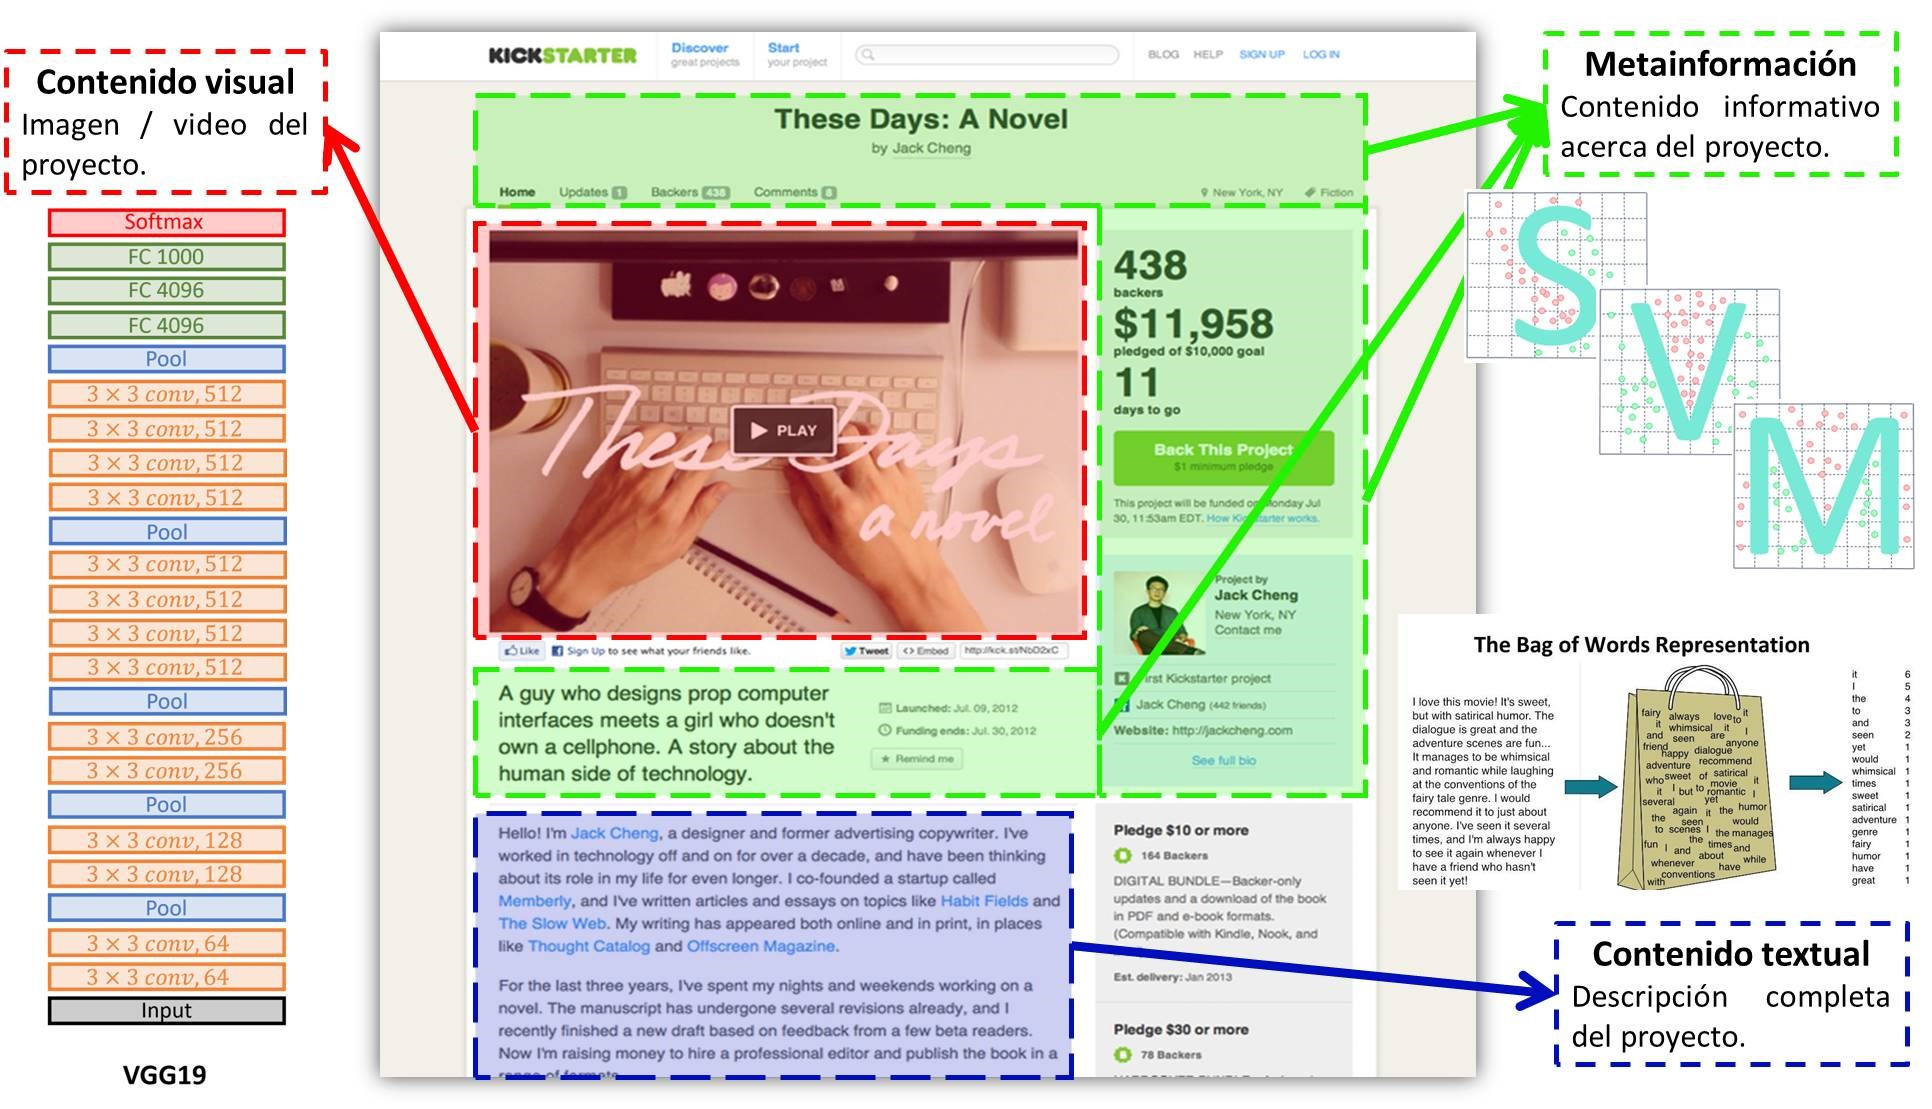
\includegraphics[width=1\textwidth]{3/figures/prototipo.jpg}
		\caption{Marco de trabajo del prototipo final. Fuente: Elaboración propia}
		\label{3:fig1}
	\end{center}
\end{figure}

\section{Población y muestra}

\subsection{Población}
La población que será considerada para el presente trabajo será de 27,251 proyectos en Kickstarter de la categoría tecnología de todas las subcategorías entre los periodos 2009-2019, en su mayoría del territorio de los Estados Unidos de América.

\subsection{Muestra}
Se distribuyeron los subconjuntos de entrenamiento y prueba en proporciones de 80\% (21,710 registros) y 20\% (5,541 registros) respectivamente (\citeauthor{pr_yuan2016textanalytics}, cuarto antecedente; \citeauthor{pr_yu2018deeplearning}, octavo antecedente; \citeauthor{pr_chen2019keywords_crowdfunding}, undécimo antecedente; \citeauthor{pr_mitra2014phrases}, duodécimo antecedente; \citeauthor{pr_sawhney2016usingLT}, decimotercer antecedente).

\subsection{Unidad de análisis}
La unidad de análisis para el presente trabajo será un proyecto en Kickstarter de la categoría tecnología de cualquier subcategoría entre los periodos 2009-2019 dentro del territorio de los Estados Unidos de América.

\section{Operacionalización de Variables}
En la Tabla \ref{3:table1} se presentan las variables usadas para el conjunto de datos final basado en contenido textual y metainformación. Estas fueron seleccionadas de acuerdo al Benchmarking aplicado a los 17 antecedentes en el Capítulo II.

\begin{table}[h!]
	\centering
	\small
	\begin{tabular}{ |m{3cm}|m{10cm}|m{2cm}|  }
		\hline
		\rowcolor{bluejean}
		\Centering \color{white}{Variable}& \Centering \color{white}{Detalle}& \Centering \color{white}{Tipo de dato}\\
		\hline
		\rowcolor{turq}
		\multicolumn{3}{c}{Variables independientes} \\
		\hline
		\textbf{goal} &	Monto de la meta de financiamiento del proyecto. &	float64 \\
		\hline
		\textbf{completeness} & Porcentaje de financiamiento o completitud. & float64 \\
		\hline
		\textbf{duration} &	Duración de la campaña (en días). &	int64 \\
		\hline
		\textbf{pledges\_num} &	Cantidad de montos disponibles para contribuir. &	int64 \\
		\hline
		\textbf{pledged} &	Monto contribuído en la campaña. &	float64 \\
		\hline
		\textbf{pledges\_median} &	Mediana de montos disponibles para contribuir. &	float64 \\
		\hline
		\textbf{description} &	Descripción del proyecto. &	object \\
		\hline
		\textbf{comments} & Comentarios de patrocinadores sobre el proyecto. & object \\
		\hline
		\rowcolor{turq}
		\multicolumn{3}{c}{Variable dependiente} \\
		\hline
		\textbf{state} & Estado de financiamiento del proyecto. & object \\
		\hline
	\end{tabular}
	\caption{Diccionario de datos del conjunto final entrenado. Fuente: Elaboración propia.}
	\label{3:table1}
\end{table}

Los autores citados por cada variable utilizada se mencionan a continuación:
\begin{itemize}
	\item \textbf{goal}: \citeauthor{pr_kamath2018suplearn} (primer antecedente), \citeauthor{pr_zhou2015projectdesc} (tercer antecedente), \citeauthor{pr_yuan2016textanalytics} (cuarto antecedente), \citeauthor{pr_chen2015predcrowd} (quinto antecedente), \citeauthor{pr_li2016predcrowd} (sexto antecedente), \citeauthor{pr_kaur2017socmedcrowd} (séptimo antecedente), \citeauthor{pr_yu2018deeplearning} (octavo antecedente), \citeauthor{pr_jin2019dayssuccess} (noveno antecedente), \citeauthor{pr_cheng2019deeplearning} (décimo antecedente), \citeauthor{pr_mitra2014phrases} (duodécimo antecedente), \citeauthor{pr_sawhney2016usingLT} (decimotercer antecedente), \citeauthor{pr_chen2013kickpredict} (decimocuarto antecedente).
	\item \textbf{completeness}: \citeauthor{pr_chen2015predcrowd} (quinto antecedente).
	\item \textbf{duration}: \citeauthor{pr_kamath2018suplearn} (primer antecedente), \citeauthor{pr_zhou2015projectdesc} (tercer antecedente), \citeauthor{pr_li2016predcrowd} (sexto antecedente), \citeauthor{pr_kaur2017socmedcrowd} (séptimo antecedente), \citeauthor{pr_yu2018deeplearning} (octavo antecedente), \citeauthor{pr_jin2019dayssuccess} (noveno antecedente), \citeauthor{pr_mitra2014phrases} (duodécimo antecedente), \citeauthor{pr_sawhney2016usingLT} (decimotercer antecedente).
	\item \textbf{pledges\_num}: \citeauthor{pr_yuan2016textanalytics} (cuarto antecedente), \citeauthor{pr_chen2015predcrowd} (quinto antecedente), \citeauthor{pr_jin2019dayssuccess} (noveno antecedente), \citeauthor{pr_mitra2014phrases} (duodécimo antecedente), \citeauthor{pr_chen2013kickpredict} (decimocuarto antecedente).
	\item \textbf{pledged}: \citeauthor{pr_kamath2018suplearn} (primer antecedente), \citeauthor{pr_li2016predcrowd} (sexto antecedente), \citeauthor{pr_chen2013kickpredict} (decimocuarto antecedente).
	\item \textbf{pledges\_median}: \citeauthor{pr_chen2015predcrowd} (quinto antecedente)*, \citeauthor{pr_jin2019dayssuccess} (noveno antecedente)*.
	\item \textbf{description}: \citeauthor{pr_kamath2018suplearn} (primer antecedente), \citeauthor{pr_zhou2015projectdesc} (tercer antecedente), \citeauthor{pr_yuan2016textanalytics} (cuarto antecedente), \citeauthor{pr_jin2019dayssuccess} (noveno antecedente), \citeauthor{pr_cheng2019deeplearning} (décimo antecedente), \citeauthor{pr_chen2019keywords_crowdfunding} (undécimo antecedente), \citeauthor{pr_mitra2014phrases} (duodécimo antecedente), \citeauthor{pr_sawhney2016usingLT} (decimotercer antecedente), \citeauthor{pr_chaichi2019nlp_3dprinting} (decimoquinto antecedente).
	\item \textbf{comments}: \citeauthor{pr_li2016predcrowd} (sexto antecedente), \citeauthor{pr_kaur2017socmedcrowd} (séptimo antecedente), \citeauthor{pr_jin2019dayssuccess} (noveno antecedente).
\end{itemize}

Si bien en los respectivos antecedentes marcados en (*) figuran el promedio de los montos disponibles para patrocinar, se usó la mediana en vez de la media ya que presentó mejor performance en los experimentos.

\section{Instrumentos de medida}


\section{Técnicas de recolección de datos}
Los conjuntos de datos recolectados para la investigación son un mix de observaciones cuantitativas (variables numéricas medibles como la meta de financiamiento, montos prometidos y duración de la campaña) y cualitativas (propaganda, descripción y comentarios del proyecto). La base de datos de la metainformación, que comprende las variables cuantitativas y propaganda del proyecto, fue consolidada luego de descargar un histórico público de 10 años de la página web “Web Robots”, fundada por los ex corporativos de TI Tomás Vitulskis y Paulius Jonaitis, y posteriormente pre-procesarla. Mientras que por el lado de la descripción y comentarios de cada proyecto, se usaron técnicas y herramientas de \textit{web scraping} a partir de los URLs. Para encontrar algunos de los papers con la información requerida más cercana, se utilizaron keywords o palabras clave como \textit{crowdfunding}, \textit{Machine Learning}, \textit{Deep Learning}, \textit{prediction}, \textit{Kickstarter}, \textit{accuracy} y \textit{projects}.


\section{Técnicas para el procesamiento y análisis de la información}



\section{Cronograma de actividades y presupuesto}
Se elaboró un cronograma de actividades de toda la investigación, mostrada en la Figura \ref{3:fig2}, contemplando desde el inicio de la misma, desarrollo, evaluación de resultados y sustentación en el mes de diciembre.
\begin{figure}[h]
	\begin{center}
		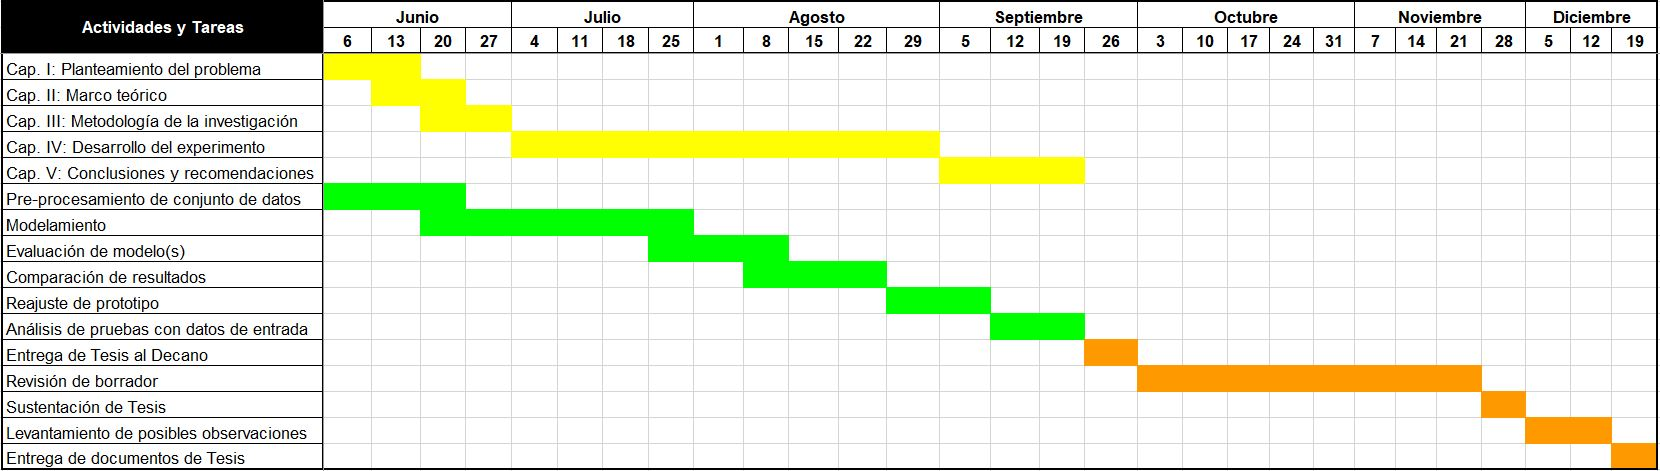
\includegraphics[width=1.1\textwidth]{3/figures/cronograma.jpg}
		\caption{Cronograma de actividades de la investigación. Fuente: Elaboración propia}
		\label{3:fig2}
	\end{center}
\end{figure}